\chapter{Erweiterte Funktionen}
In diesem Kapitel werden nun Funktionen beschrieben, die über die Grundausstattung der Web-App hinaus gehen, um diese zu erweitern und produktiver zu gestalten. 

\section{Statistiken}
Da eine Auswertung der eingegebenen Daten für Veranstaltungen unabdinglich ist, wurde ein weiterer Controller implementiert, welcher sämtliche speziellen Felder der Events aus der Datenbank abfragt und diesen dann die Werte der einzelnen Benutzer zuweist.\par

Im View wird dann eine grafische Auswertung gestartet, die mit Hilfe von Google Charts ansehnliche Graphen generiert, wo es Sinn ergibt und vergleichbare Werte von den Benutzern hinterlegt wurden. Außerdem gibt es allgemeine Statistiken, die die Veranstaltungen untereinander vergleichen und man so einen schnellen Überblick über die angelegten Events erhält.

\section{Lokalisierung von Clients}
Um die eingetragenen Helfer in dieser Webanwendung besser koordinieren zu können, wurde ein Modul implementiert, welches im Hintergrund der Web-App läuft und die aktuelle Position des Endgeräts über eine SSL verschlüsselte Verbindung an den Server übermittelt. Unter der Voraussetzung, dass der Client diesem Vorgang zustimmt, sind dem Server damit die Positionen der eingeloggten Benutzer bekannt. Diese Positionsdaten können dann von der Anwendung ausgewertet und in einer Karte von Google Maps angezeigt werden.\par

Jeder Client kann auf diese Weise die Positionen der anderen Helfer sehen. Der Vorteil liegt klar auf der Hand: eine zentral eingerichtete Verwaltung kann mit einem Blick sehen, wer sich an welcher Stelle auf dem Gelände befindet. So können Wege optimiert und gezielt Aufgaben verteilt werden, da ortsnahe Helfer die entsprechenden Aufgaben übernehmen können. Die kurzen Wege sorgen dann dafür, dass eine höhere Nutzung der Ressourcen (hier: die Helfer) möglich ist.\par

Eine wichtige Anforderung an diese Funktion ist, dass die Daten schnell ausgetauscht werden. Wenn zwischen den Updates der Positionen zu viel Zeit vergeht, ist die aktuelle Position nicht mehr aktuell und damit nicht mehr relevant.\par

Wie findet der Austausch der Positionen denn nun statt? Da es sich hier um sensible Daten handelt, ist eine sichere Übertragung Grundvoraussetzung. Allerdings steht im W3C Working Draft von HTML5, dass keine sichere, verschlüsselte Peer to Peer Verbindung mit HTML5 möglich ist \cite{w3cworkingdraft}. Im aktuellen Draft wurde auch keine sichere Verbindung definiert und es ist auch bisher keine vorgesehen \cite{w3ccurrent}.\\
Also liegt nahe weitere Techniken zu betrachten, welche einen sicheren Austausch von Daten zwischen Clients über einen Server ermöglichen.

\section{Echtzeitaktualisierung durch WebSockets}
Das wohl spannendste Thema dieser Arbeit ist die Echtzeitaktualisierung im Hintergrund der Web-App. Mehrere Möglichkeiten sind dafür gegeben, wobei einige besser geeignet sind als andere.

\subsection{Vor HTML5: Benutzung von Polling}
Für den Datenverkehr von Internetseiten wird HTTP benutzt, welches die wechselseitige Datenübermittlung \emph{Halbduplex} verwendet. So erfolgt der Datenverkehr nur in eine Richtung zur gleichen Zeit: der Client schickt eine Anfrage an den Server und dieser übermittelt danach die Antwort \cite[S. 5]{ws}. Das hat wiederum zur Folge, dass es relativ ineffizient ist, da man mit jeder Anfrage stets die Antwort des Servers abwarten muss.\par

\begin{figure}[!ht]
	\centering
	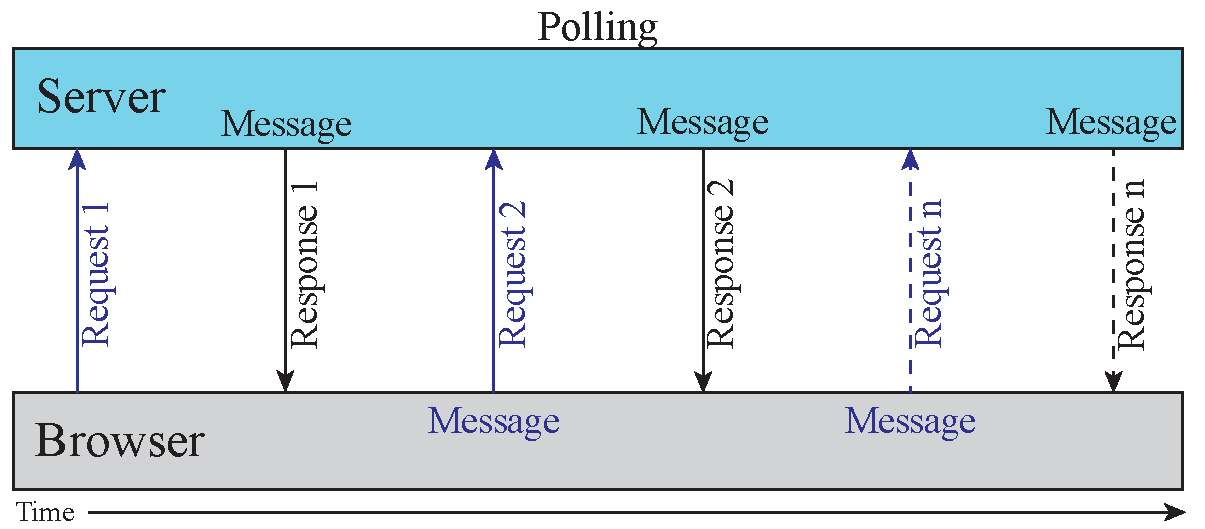
\includegraphics[width=15cm]{fig/polling}
	\caption{Datenaustausch mittels HTTP Request / Response beim Polling {\cite[S. 7]{ws}}}
\end{figure}

Vor diesem technischen Hintergrund wurde Polling entwickelt, bei dem in einem zeitlich bekannten Intervall eine Anfrage an den Server geschickt wird mit der Bitte um Aktualisierung. Diese Technik ist sehr attraktiv, wenn die zeitlichen Abstände der Aktualisierung der Daten bekannt ist, allerdings sind Echtzeitdaten schlecht vorhersehbar. Dadurch ist Polling nicht die richtige Wahl für dieses Projekt, weil es auf eine wirkliche Echtzeitaktualisierung ankommt.\par

\subsection{Einführung in WebSockets}
Mit der HTML5-Spezifikation wurden \emph{WebSockets} eingeführt, welche eine Vollduplex, bidirektionale, Single-Socket Verbindung ermöglichen \cite[S. 7]{ws}. Eine Anfrage öffnet die Verbindung zum WebSocket Server und kann beliebig lange offen gehalten werden, wobei zu jeder Zeit Daten zwischen Client und Server ausgetauscht werden. Dieser erste Handshake erfolgt über HTTP/1.1 und ähnelt dem zum Aufruf einer Homepage.
\\
\begin{lstlisting}[captionpos=b, caption=HTTP Request vom Client {\cite[S. 6]{rfc6455:handshake}}]
  GET / HTTP/1.1
  Host: server.example.com
  Origin: http://www.example.com
  Sec-WebSocket-Key: 7+C600xYyb0v2zmJ69RQsw==
  Sec-WebSocket-Version: 13
  Upgrade: websocket
\end{lstlisting}

Mit \emph{Upgrade: websocket} wird signalisiert, dass der Client eine WebSocket-Verbindung zum Server aufbauen möchte. Der entsprechende WebSocket Server reagiert darauf mit dem HTTP-Statuscode \emph{101 Switching Protocols}, womit er bestätigt, dass er mit dem Wechsel des Protokolls einverstanden ist.
\\
\begin{lstlisting}[captionpos=b, caption=HTTP Response vom Server {\cite[S. 8]{rfc6455:handshake}}]
  101 Switching Protocols
  Connection: Upgrade
  Sec-WebSocket-Accept: fYoqiH14DgI+5y1EMwM2sOLzOi0=
  Upgrade: WebSocket
\end{lstlisting}

Der kryptische Schlüssel \emph{Sec-WebSocket-Accept} muss vom Server berechnet und zurückgegeben werden und zeigt damit, dass er das WebSocket Protokoll versteht. Ab diesem Zeitpunkt ist der Handshake abgeschlossen und die WebSocket-Verbindung wurde aufgebaut.\par

Nun kommen die Vorteile von WebSockets zur Geltung: nach erstmaligem Aufbau der Verbindung bleibt diese geöffnet und zu jedem Zeitpunkt können Client und Server die Vollduplex Verbindung nutzen, um Daten miteinander auszutauschen. Das verringert Latenzzeiten (die Pakete werden direkt zugestellt, da der Server auf keinen Request vom Client warten muss), den Traffic (der Overhead ist deutlich geringer, nur ein Handshake zu Beginn erforderlich) und die CPU-Leistung der Server (der Austausch der Daten ist einfacher gestaltet als beim Polling o.Ä.).

\begin{figure}[!ht]
	\centering
	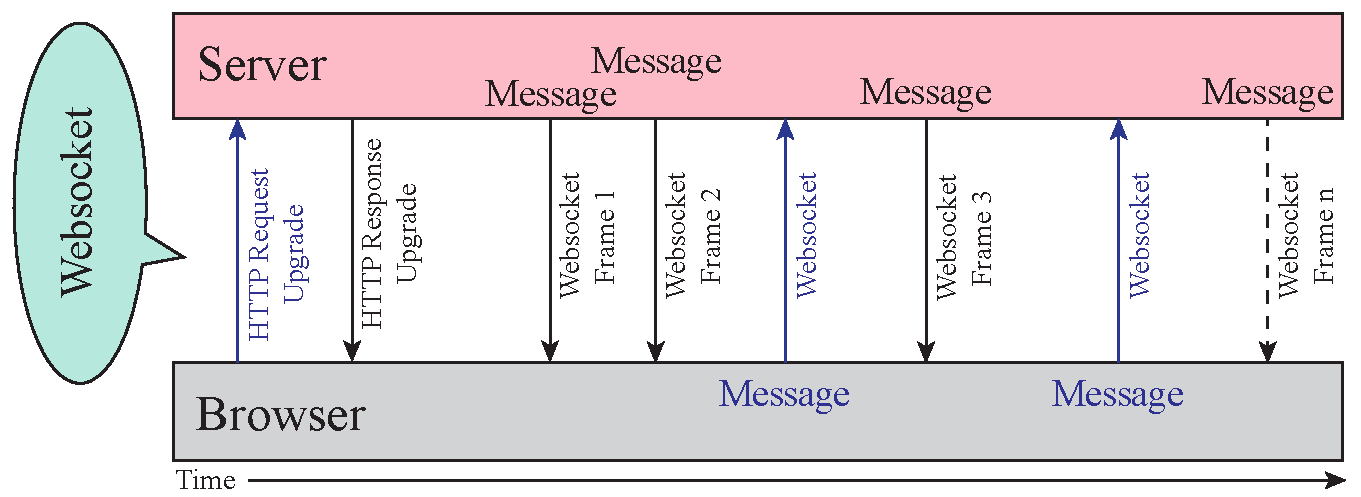
\includegraphics[width=15cm]{fig/websockets}
	\caption{Aufbau einer WebSocket Verbindung. Danach können beliebig Nachrichten in beide Richtungen (gleichzeitig) übermittelt werden}
\end{figure}

\subsection{Implementierung der Echtzeitaktualisierung}
Im ersten Ansatz dieser Arbeit wurde der WebSocket-Server auf Basis von \emph{node.js}, einem serverseitigem JavaScript Framework für Server, implementiert. Das verlief aufgrund der einfachen Handhabung von WebSockets und der guten Unterstützung von HTML5 problemlos. Jedoch wurden zu diesem Zeitpunkt weder verschlüsselte Verbindungen noch Broadcasting unterstützt. Daher war dies ungeeignet, weil sensible Daten, wie die Standorte der Clients, nicht im Klartext verschickt werden sollten.\\
Außerdem ist ein Broadcasting-Funktion notwendig, die den bestehenden Sockets bei Aktualisierung einer Position sofort die neuen Koordinaten übermittelt.\par

Die Implementierung beider Funktionen hätte den Rahmen dieser Arbeit überschritten, weshalb serverseitig das Open Source Modul \emph{socket.io} für node.js verwendet wird, welches sämtliche benötigten Dienste bereitstellt und dabei noch einen Fallback zur Verfügung stellt, wodurch auch älteren Browsern ohne HTML5 Unterstützung eine websocketähnliche Verbindung ermöglicht wird.\par

Clientseitig wurde eine Routine in JavaScript entwickelt, welche im Hintergrund der Web-App ausgeführt wird. Dieses Skript verbindet sich mit dem WebSocket Server, schickt initial die aktuellen Koordinaten (unabhängig davon, welcher View gerade angezeigt wird) und wartet auf eingehende Nachrichten oder auf eine Änderung der eigenen Position. Bewegt sich der Client werden automatisch die Koordinaten GoogleMaps-kompatibel in Form von Latitude und Longitude an den WebSocket Server übermittelt.\\
Erhält der Server so eine Nachricht, aktualisiert er seine Datenbank von Standorten der Clients und schickt per Broadcast eine Nachricht an alle verbundenen Clients. So erhalten die Endgeräte in Echtzeit eine Aktualisierung aller Positionen.\par

Beendet ein Client die Verbindung oder erhält der Server keine Aktualisierungen mehr, so wird sein letzter Standort noch 15 Minuten gespeichert und dann auf allen Endgeräten gelöscht. Zu keiner Zeit werden Daten protokolliert oder länger als nötig gespeichert.\par

\paragraph{Schwierigkeit beim Wechseln oder Neuladen eines Views}\ \\ \
Ein Problem, welches bei der Nutzung von WebSockets (kurz: WS) auftrat, war der Übergang zwischen den einzelnen Seiten: Wird eine Seite gewechselt, so wird die WebSocket Verbindung geschlossen, die nächste Seite per HTTP Request angefordert und eine neue Verbindung zum WS Server aufgebaut. Also wird mit jedem Wechsel ein neuer Socket erstellt, den der Server neu zu den bestehenden Daten des Clients referenzieren muss.\\
Damit ist nun durch neue Assoziationen von Referenzen ein Wechsel zwischen den Views möglich, ohne dabei Werte wie Positionen des Clients zu verlieren, möglich.

\paragraph{Entwicklung eines eigenen Protokolls zur Kommunikation über WebSockets}\ \\ \
Um bestimmte Funktionen auf dem Server anzusprechen, wurde ein einfaches Protokoll entwickelt, welches angibt, um welchen Inhalt es sich bei der Nachricht handelt. So haben alle Nachrichten, die zwischen Client und Server ausgetauscht werden, ein bestimmtes Format und ein Feld \emph{type}, welches aktuell folgende Werte annehmen kann:

\begin{itemize}
	\item[] \emph{location:} enthält Latitude und Longitude des Clients
	\item[] \emph{syn:} enthält eine Signatur, die überprüft wird
	\item[] \emph{subscribe:} abonniert bestimmte Events, dazu später mehr
	\item[] \emph{publish:} signalisiert eine Änderung an der Datenbank
\end{itemize}

Der socket.io Server wertet diese Fälle über ein \emph{Switch-Case-Statement} aus und ruft entsprechende Methoden zur weiteren Verarbeitung auf.

\subsection{Authentifizierung eines Clients beim WebSocket Server}
In der anfänglichen Implementierung der Skripte für die Kommunikation zwischen Client und Server war es noch möglich die Positionsdaten von Benutzern abzufangen, indem man sich simpel für diese beim WS Server ausgegeben hat. Wenn der Server eine Nachricht bekommen hat mit Inhalt \emph{Ich bin \glqq BenutzerXY\grqq{}}, so wurde diese Verbindung in die Liste der verbundenen Sockets des Accounts eingetragen und so konnte der \glqq Angreifer\grqq{} alle Standorte der Clients beim nächsten Broadcast empfangen.\par

Über das Public-Key-Verschlüsselungsverfahren wurde dann eine serverseitige Methode implementiert, die bei der ersten Initialisierung der Meißner-Webanwendung mit \emph{openssl} je einen öffentlichen und privaten RSA Schlüssel erstellt. Mit diesem privaten Schlüssel wird eine Signatur der Nachricht des Typs \emph{syn} erstellt, an die Nachricht angehangen und dem WebSocket Server zugeschickt.\\
Socket.io erkennt ein \emph{syn} und die Signatur, öffnet den öffentlichen Schlüssel der Webanwendung und überprüft so die Signatur. Sofern diese gültig ist, wird der Client, der die Nachricht übermittelt hat, in die Liste der gültigen Clients eingefügt.\par

Dadurch ist garantiert, dass die Signatur der Web-App wirklich nur von dieser Anwendung stammt und es sich damit um einen normalen Benutzer handelt. Andernfalls wird die Verbindung mit der Fehlermeldung \emph{unauthorized} abgewiesen.\par

Alle weiteren Typen von Nachrichten können nun durch eine einfache \emph{default: deny} Regel alle einkommenden Nachrichten verwerfen, die von Verbindungen stammen, welche vorher keine Authentifizierung beim Server vollzogen haben. Das spart Rechenleistung, denn es muss nur ein kurzer Vergleich der Objektreferenz erledigt werden.\par


\subsection{Entwurfsmuster: Publish/Subscribe}
Da die Meißner App nun über eine Echtzeitaktualisierung verfügt, wird diese genutzt, um das \emph{Publish/Subscribe Muster} anzuwenden.



















